\documentclass{beamer}

\usepackage[T1,T2A]{fontenc}
\usepackage[utf8]{inputenc}

\usepackage{amsmath}
\usepackage{wrapfig}

\usepackage{bsuslides}

% \graphicspath{ {img/} }

\title{АНАЛИЗ И РАЗРАБОТКА РАСПРЕДЕЛЁННОЙ АРХИТЕКТУРЫ ЭКСПЛУАТАЦИИ НЕЙРОННЫХ СЕТЕЙ\\}
\subtitle{Дипломная работа}
\author{Ларин Егор Сергеевич}
\institute[БГУ]{Белорусский государственный университет \\ ФПМИ, КТС, 4 курс \\ руководитель: старший преподаватель Шолтанюк С. В.}
\date{Минск, 2024}

%\nofiles
\begin{document}

\frame{\titlepage}

\begin{frame}
	\frametitle{Введение}
	\begin{itemize}
		\item В последние годы микросервисная архитектура значительно приобретает популярность в области разработки программного обеспечения. 
		\item Использование микросервисной помогает решить вопросы масштабируемости.
		\item Внедрение микросервисов порождает другие проблемы, которые необходимо решать с помощью современных инструментов.
	\end{itemize}
\end{frame}

\begin{frame}
	\frametitle{Микросервисы}
	\begin{enumerate}
		\item Нет формального определения.
		\item Одним из подходов является проверка соответствия критериям масштабируемости.
		\item Низкая связность.
		\item Зачастую начинают использовать слишком рано.
	\end{enumerate}
\end{frame}

\begin{frame}
	\frametitle{Куб масштабируемости}
	\centering
	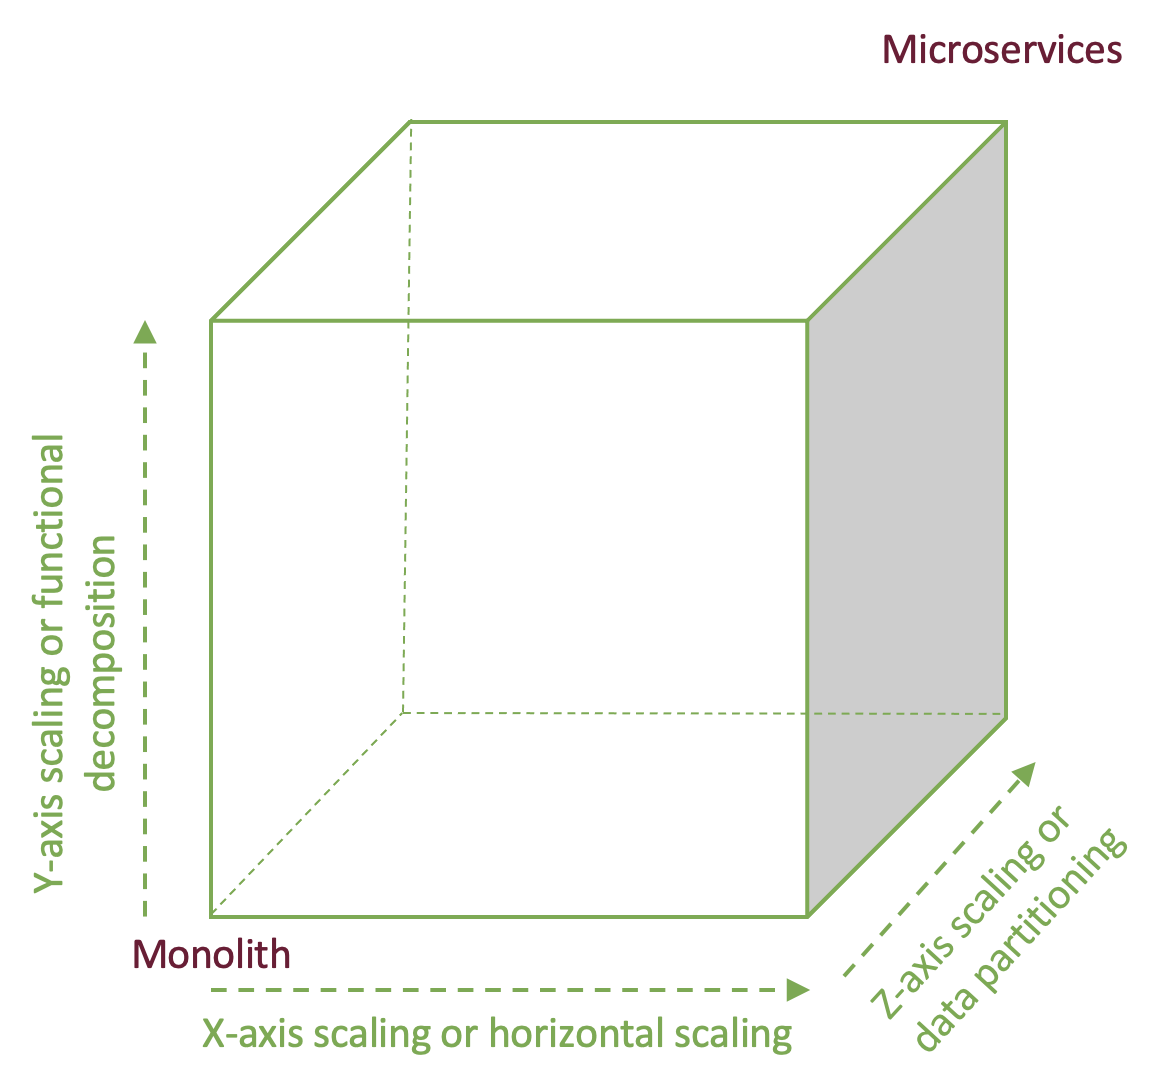
\includegraphics[height=7cm]{img/cube.png}
\end{frame}

\begin{frame}
	\frametitle{Распределенный монолит}
	\centering
	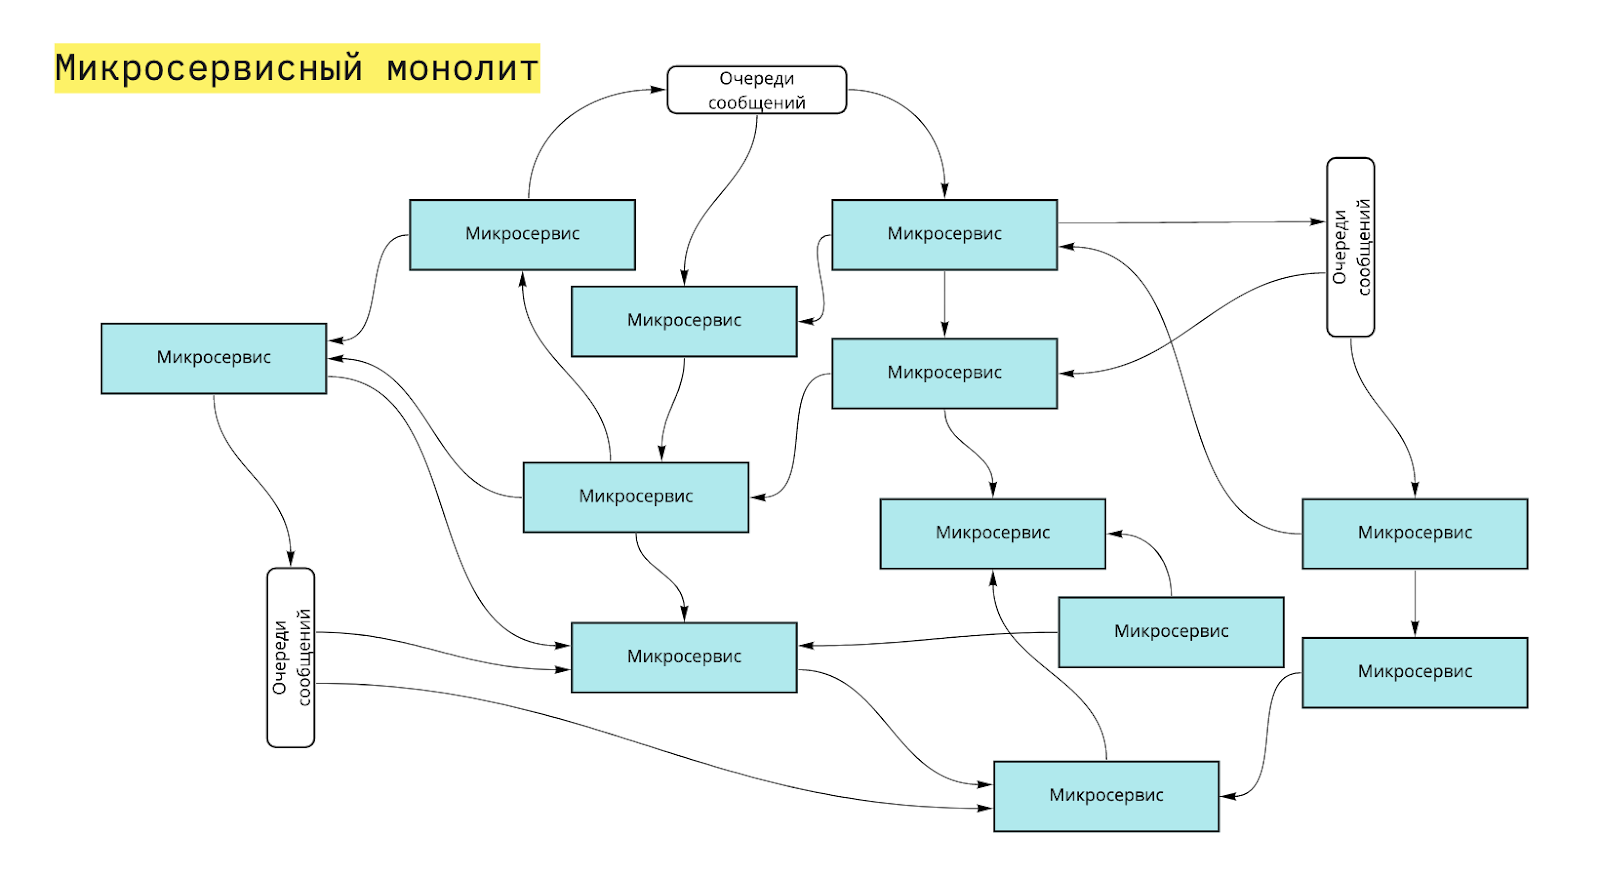
\includegraphics[height=5cm]{img/mon.png}
\end{frame}

\begin{frame}
	\frametitle{Сервис для генерации изображений}
	\begin{itemize}
		\item Gateway.
		\item Internal Backend.
        \item Sidecar.
	\end{itemize}
\end{frame}

\begin{frame}
	\frametitle{Схема архитектуры}
	\centering
	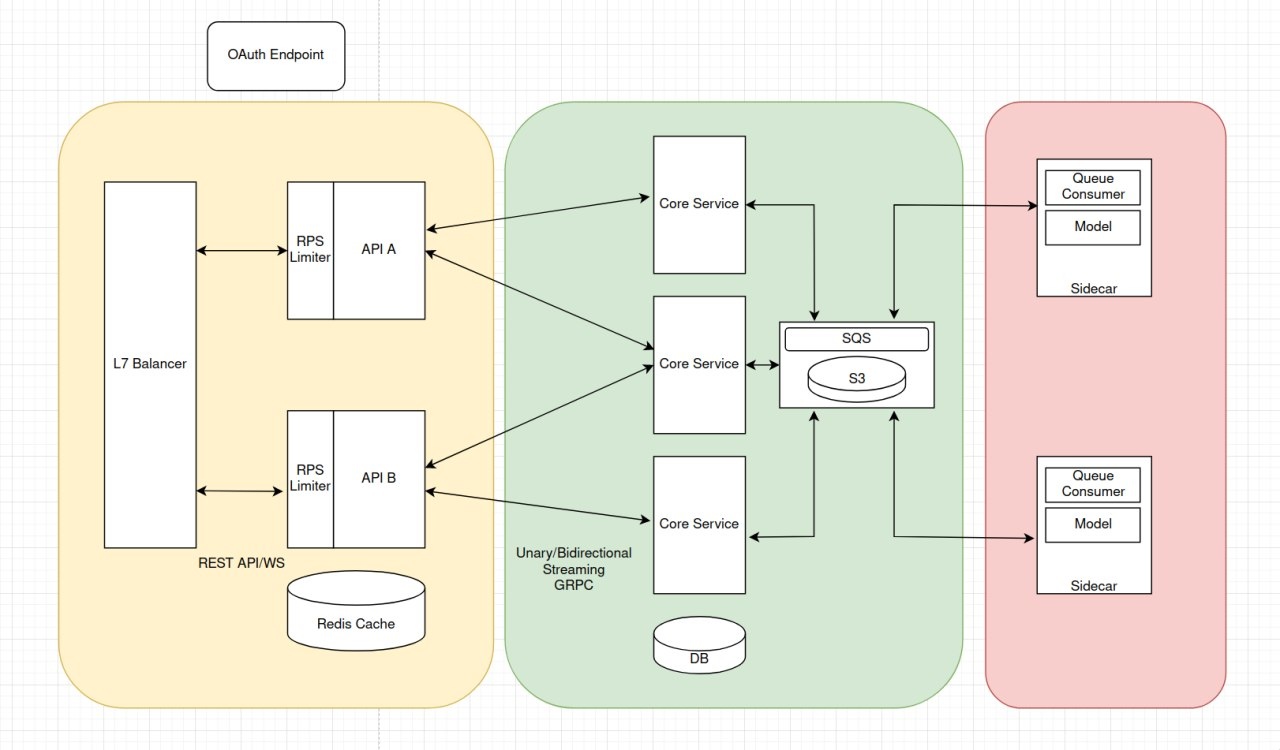
\includegraphics[height=7cm]{img/design.png}
\end{frame}

\begin{frame}
	\frametitle{Native Sidecar}
	\centering
	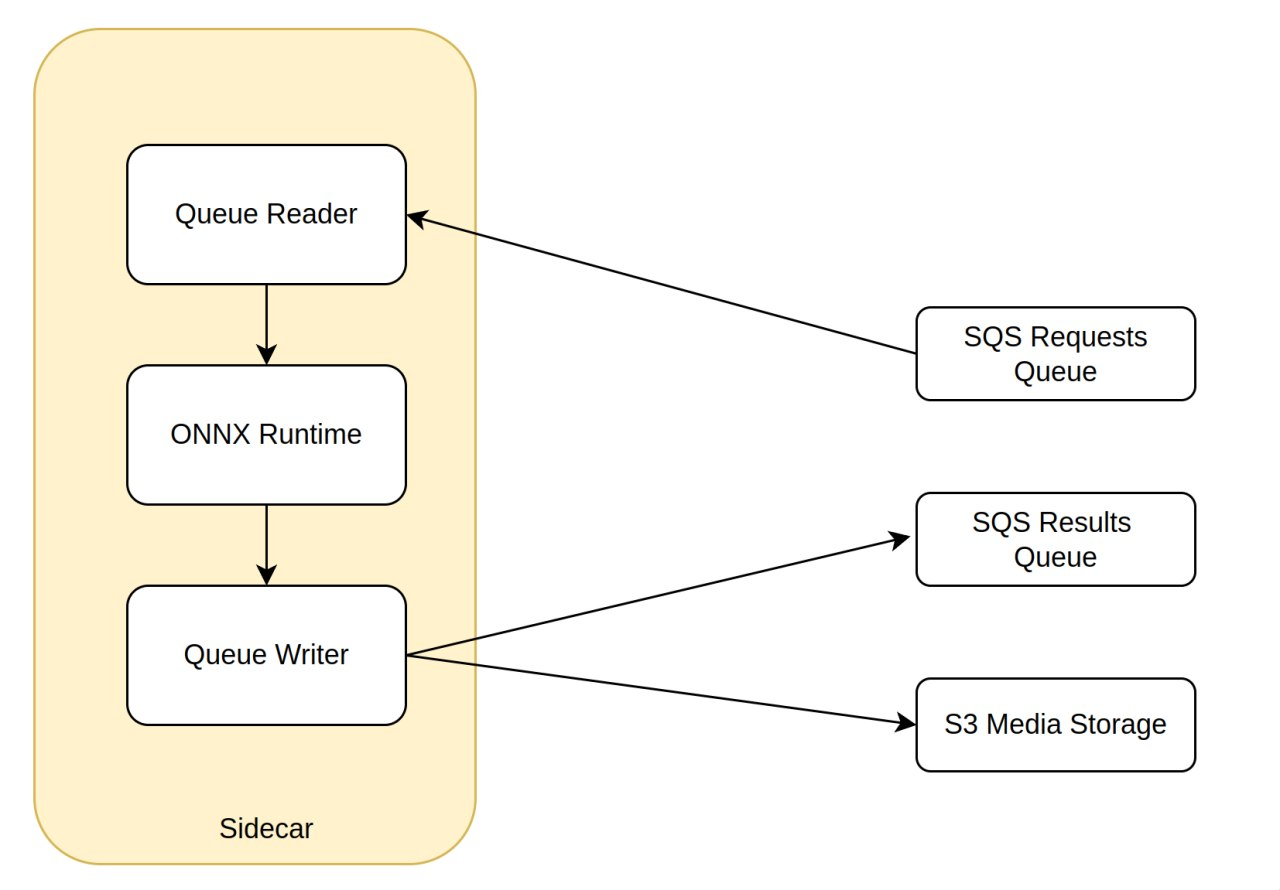
\includegraphics[height=5cm]{img/side1.jpg}
\end{frame}

\begin{frame}
	\frametitle{HTTP Sidecar}
	\centering
	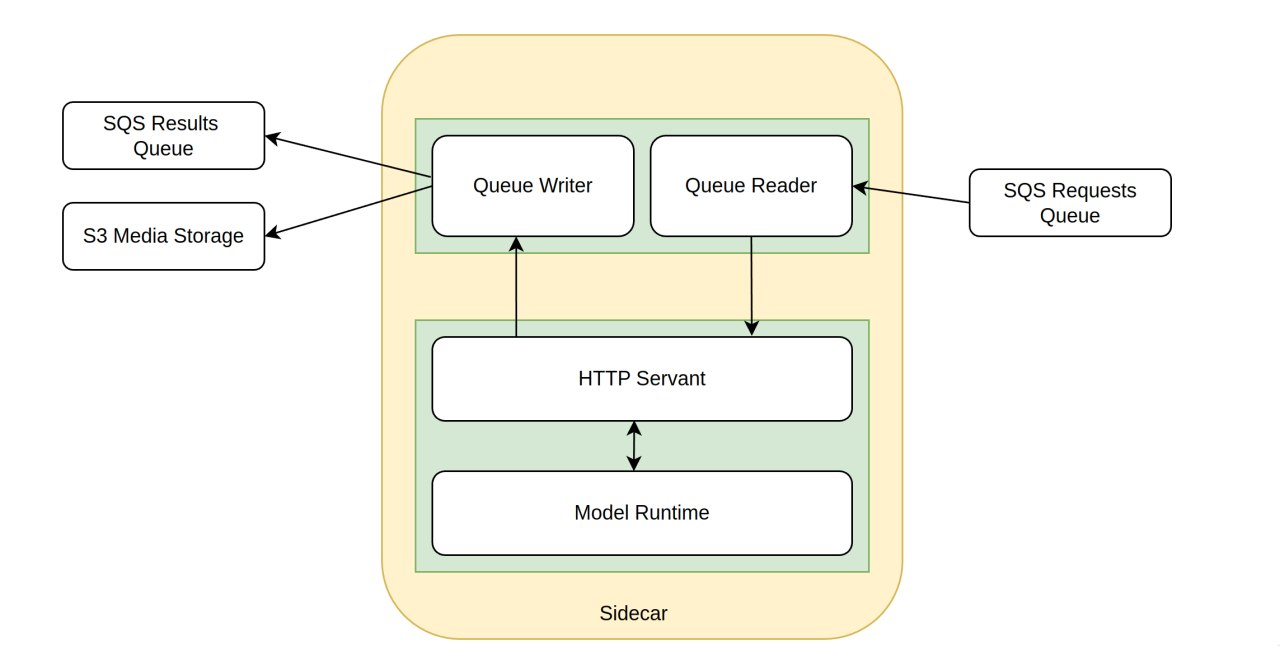
\includegraphics[height=5cm]{img/side2.jpg}
\end{frame}

\begin{frame}
	\frametitle{UDS Sidecar}
	\centering
	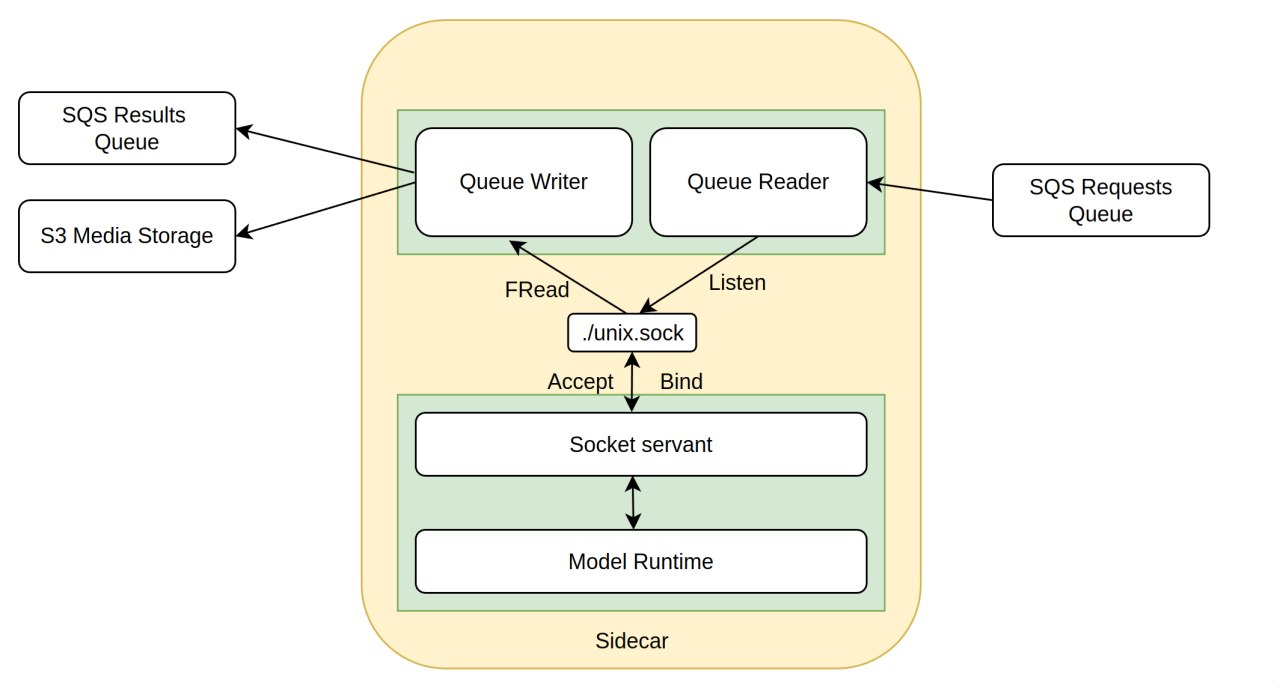
\includegraphics[height=5cm]{img/side3.jpg}
\end{frame}



\begin{frame}
	\frametitle{Заключение}
	\begin{itemize}
	\item В ходе работы было рассмотрено понятие микросервисной архитектуры и произведен обзор имеющихся средств и методологий разработки, применяющихся для коммуникации веб-сервисов.
	\item Результатом работы стала разработка программного обеспечения для генерации изображений с помощью нейронной сети с сетевым интерфейсом. 
	\item Рассмотрены подходы общения разных процессов и проанализированы достоинства и недостатки каждого из методов.
	\end{itemize}
\end{frame}

\begin{frame}
	\frametitle{Источники}
	\begin{enumerate}
		\item Микросервисы: паттерны разработки и рефакторинга / Крис Ричардсон. - Санкт-Петербург [и др.] : Питер, Прогресс книга, 2020. - 542 с. -  (Библиотека программиста). 
		\item Высоконагруженные приложения: программирование, масштабирование, поддержка: [перевод с английского] / Мартин Клеппман. - Санкт-Петербург [и др.] : Питер, Прогресс книга, 2018. - 637 с. -  (Бестселлеры O'Reilly). 
		\item Marek Bolanowski, Kamil Zak, Andrzej Paszkiewicz, Maria Ganzha, Marcin Paprzycki, Piotr Sowinski, Ignacio Lacalle, and Carlos E. Palau. Eficiency of REST and gRPC Realizing Communication Tasks in Microservice-Based Ecosystems. IOS Press, September 2022..
	\end{enumerate}
\end{frame}

\end{document} 
